\documentclass[12pt]{article}
\usepackage{amsmath}
\usepackage{graphicx}
\usepackage{hyperref}
\usepackage{listings}
\usepackage{color}
\usepackage{pythonhighlight}


\title{Operating System Course Report - First Half of the Semester}
\author{A class}
\date{\today}

\begin{document}

\maketitle
\newpage

\tableofcontents
\newpage

\section{Introduction}
This report summarizes the topics covered during the first half of the Operating System course. It includes theoretical concepts, practical implementations, and assignments. The course focuses on the fundamentals of operating systems, including system architecture, process management, CPU scheduling, and deadlock handling.

\section{Course Overview}
\subsection{Objectives}
The main objectives of this course are:
\begin{itemize}
    \item To understand the basic components and architecture of a computer system.
    \item To learn process management, scheduling, and inter-process communication.
    \item To explore file systems, input/output management, and virtualization.
    \item To study the prevention and handling of deadlocks in operating systems.
\end{itemize}

\subsection{Course Structure}
The course is divided into two halves. This report focuses on the first half, which covers:
\begin{itemize}
    \item Basic Concepts and Components of Computer Systems
    \item System Performance and Metrics
    \item System Architecture of Computer Systems
    \item Process Description and Control
    \item Scheduling Algorithms
    \item Process Creation and Termination
    \item Introduction to Threads
    \item File Systems
    \item Input and Output Management
    \item Deadlock Introduction and Prevention
    \item User Interface Management
    \item Virtualization in Operating Systems
\end{itemize}

\section{Topics Covered}

\subsection{Basic Concepts and Components of Computer Systems}
This section explains the fundamental components that make up a computer system, including the CPU, memory, storage, and input/output devices.

\subsection{System Performance and Metrics}
This section introduces various system performance metrics used to measure the efficiency of a computer system, including throughput, response time, and utilization.

\subsection{System Architecture of Computer Systems}
Describes the architecture of modern computer systems, focusing on the interaction between hardware and the operating system.

\subsection{Process Description and Control}
Processes are a central concept in operating systems. This section covers:
\begin{itemize}
    \item Process states and state transitions
    \item Process control block (PCB)
    \item Context switching
\end{itemize}

\subsection{Scheduling Algorithms}
This section covers:
\begin{itemize}
    \item First-Come, First-Served (FCFS)
    \item Shortest Job Next (SJN)
    \item Round Robin (RR)
\end{itemize}
It explains how these algorithms are used to allocate CPU time to processes.

\subsection{Process Creation and Termination}
Details how processes are created and terminated by the operating system, including:
\begin{itemize}
    \item Process spawning
    \item Process termination conditions
\end{itemize}

\subsection{Introduction to Threads}
This section introduces the concept of threads and their relation to processes, covering:
\begin{itemize}
    \item Single-threaded vs. multi-threaded processes
    \item Benefits of multithreading
\end{itemize}

\begin{figure}[h]
    \centering
    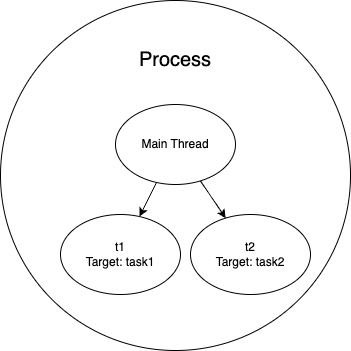
\includegraphics[width=0.5\textwidth]{/Users/khawaritzmi/Unhas/os_report_mid2024/a_class/asset/example.png}  % Sesuaikan nama file dan ukurannya
    \caption{Ini adalah gambar contoh dari multithreading.}
    \label{fig:contoh_gambar}
\end{figure}

Seperti yang terlihat pada Gambar \ref{fig:contoh_gambar}, inilah cara menambahkan gambar dengan keterangan.

\subsection{File Systems}
File systems provide a way for the operating system to store, retrieve, and manage data. This section explains:
\begin{itemize}
    \item File system structure
    \item File access methods
    \item Directory management
\end{itemize}

\subsection{Input and Output Management}
Input and output management is key for handling the interaction between the system and external devices. This section includes:
\begin{itemize}
    \item Device drivers
    \item I/O scheduling
\end{itemize}

\subsection{Deadlock Introduction and Prevention}
Explores the concept of deadlocks and methods for preventing them:
\begin{itemize}
    \item Deadlock conditions
    \item Deadlock prevention techniques
\end{itemize}

\subsection{User Interface Management}
This section discusses the role of the operating system in managing the user interface. Topics covered include:
\begin{itemize}
    \item Graphical User Interface (GUI)
    \item Command-Line Interface (CLI)
    \item Interaction between the user and the operating system
\end{itemize}

\subsubsection{Karakteristik User Interface}
Dalam mendesain antarmuka pengguna, terdapat beberapa karakteristik yang harus dipertimbangkan agar pengguna mendapatkan pengalaman yang optimal. Karakteristik tersebut adalah:

\begin{itemize}
    \item \textbf{Jelas (\textit{Clarity)}}: Antarmuka yang jelas memudahkan pengguna memahami fungsionalitas dan informasi yang disajikan \cite{nielsen1995}.
    \item \textbf{Singkat \textit{(Conciseness)}}: Penyajian informasi yang tidak bertele-tele meningkatkan efektivitas penggunaan antarmuka \cite{shneiderman1997}.
    \item \textbf{Konsisten \textit{(Consistency)}}: Konsistensi dalam tampilan dan fungsi antarmuka membantu pengguna menguasai sistem dengan lebih cepat \cite{nielsen2000}.
    \item \textbf{Responsif \textit{(Responsiveness)}}: Responsivitas penting agar pengguna merasa antarmuka dapat diandalkan \cite{holtzblatt2005}.
    \item \textbf{Menarik \textit{(Attractiveness)}}: Tampilan yang menarik secara visual meningkatkan kepuasan pengguna \cite{tractinsky1997}.
    \item \textbf{Familiar \textit{(Familiarity)}}: Menggunakan elemen yang sudah dikenal pengguna mempermudah adaptasi dengan antarmuka \cite{norman1988}.
    \item \textbf{Efisien \textit{(Efficiency)}}: Antarmuka harus memfasilitasi tugas pengguna dengan cepat dan mudah \cite{nielsen1993}.
\end{itemize}

\subsubsection{Contoh User Interface}

Dalam dunia desain antarmuka pengguna (UI), tren terus berkembang untuk memberikan pengalaman yang lebih interaktif dan menyenangkan. Beberapa contoh tren UI yang sedang populer saat ini meliputi:

\paragraph{Advance Cursor Interactions}
\textit{Advance cursor interactions} melibatkan penggunaan kursor untuk lebih dari sekadar penunjuk sederhana. UI ini memungkinkan kursor merespons interaksi pengguna dengan efek seperti perubahan bentuk, ukuran, atau warna, memberikan pengalaman yang lebih interaktif dan imersif \cite{busche2020}. Efek ini meningkatkan keterlibatan pengguna dengan membuat elemen UI terasa lebih responsif dan hidup.

\paragraph{Complex \& Animated Gradients}
Gradien kompleks dengan animasi memberikan tampilan yang dinamis pada antarmuka pengguna. Penggunaan berbagai warna dengan perpindahan halus dan animasi lembut menciptakan visual yang menarik dan memberikan kesan modern \cite{sutton2020}. Gradien ini sering digunakan untuk memberikan kedalaman dan menciptakan ilusi gerakan di dalam UI.

\paragraph{Bold Color Choices}
Pemilihan warna yang tegas dan mencolok semakin populer di desain UI. Warna-warna berani memberikan kontras yang kuat dan menciptakan suasana yang energik dan penuh semangat. Desain dengan warna tegas juga dapat menarik perhatian pengguna dan memandu mereka ke bagian penting dari antarmuka \cite{coleman2021}.

\paragraph{Focus on Typography}
Fokus pada tipografi dalam UI menekankan pentingnya penggunaan font yang tepat untuk menyampaikan pesan dengan jelas. Ukuran huruf yang besar dan pilihan font yang kuat membantu meningkatkan keterbacaan serta estetika antarmuka \cite{tschichold1995}. Tipografi yang baik juga memperkuat identitas merek dan meningkatkan pengalaman pengguna secara keseluruhan.

\paragraph{Dark Mode}
\textit{Dark mode} menjadi tren populer karena mengurangi ketegangan mata saat pengguna menggunakan aplikasi dalam kondisi pencahayaan rendah. Dengan menggunakan warna gelap sebagai latar belakang dan warna terang untuk teks, mode ini juga membantu menghemat energi pada perangkat dengan layar OLED \cite{ricker2021}. Selain itu, dark mode memberikan tampilan yang lebih elegan dan modern pada UI.
\begin{figure}[h]
    \centering
    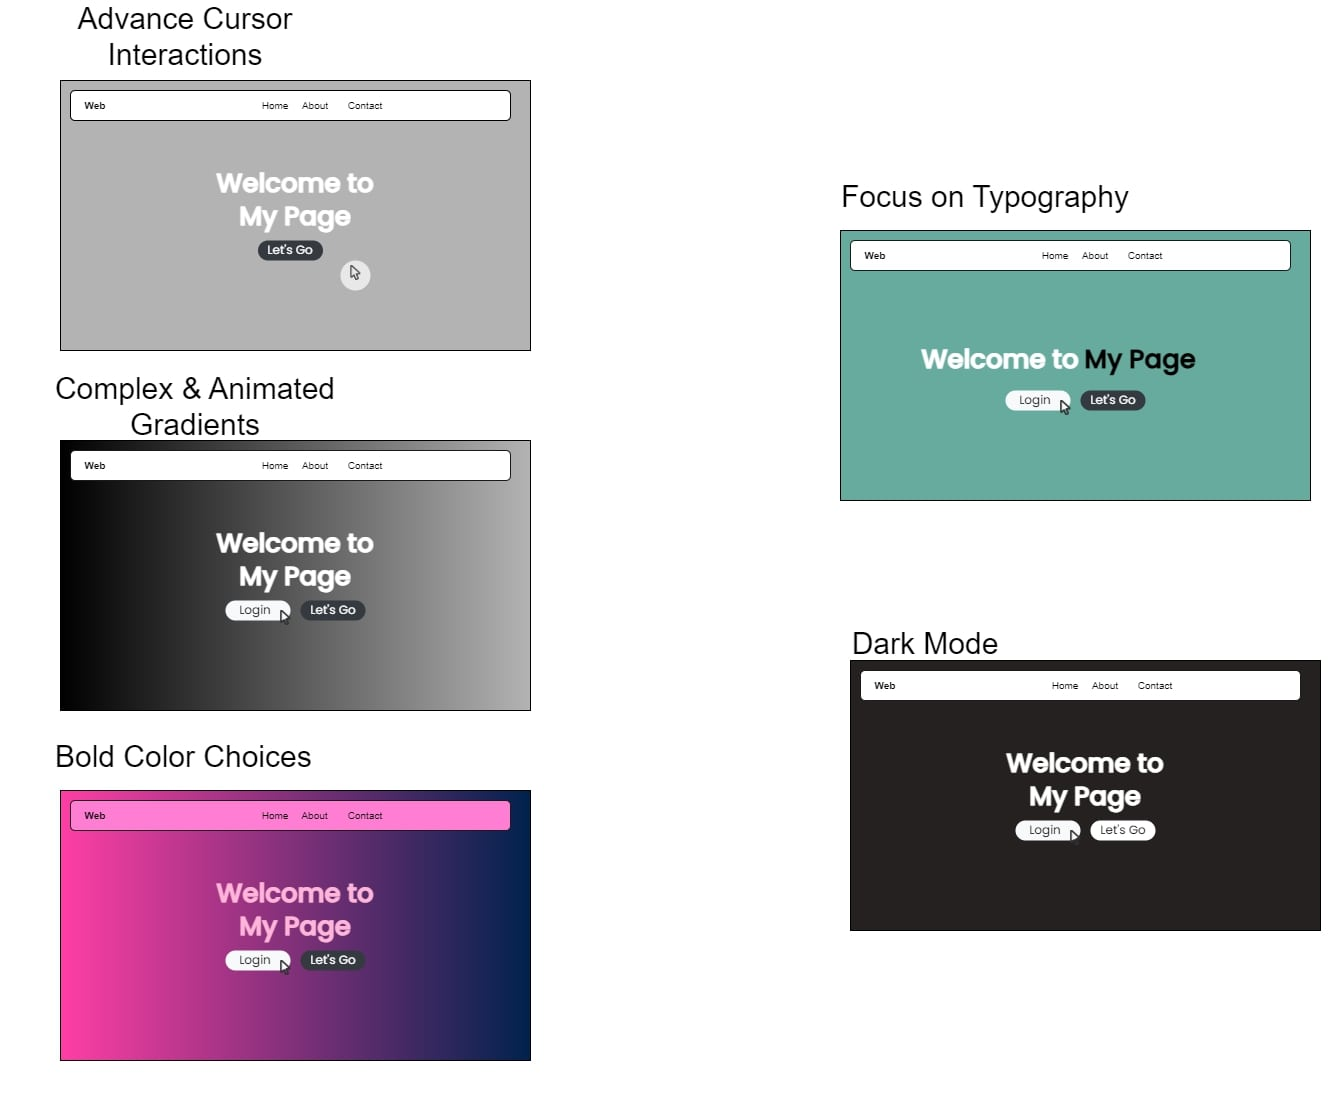
\includegraphics[width=0.8\textwidth]{asset/ContohUI.drawio (1).jpg}
    \caption{Contoh desain UI.}
    \label{fig:contoh_ui}
\end{figure}

\subsection{Virtualization in Operating Systems}
Virtualization allows multiple operating systems to run concurrently on a single physical machine. This section explores:
\begin{itemize}
    \item Concept of virtualization
    \item Hypervisors and their types
    \item Benefits of virtualization in modern computing
\end{itemize}

\section{Assignments and Practical Work}
\subsection{Assignment 1: Process Scheduling}
Students were tasked with implementing various process scheduling algorithms (e.g., FCFS, SJN, and RR) and comparing their performance under different conditions.
\subsubsection{Group 1}
\begin{python}
    class Process:
    def init(self, pid, arrival_time, burst_time):
        self.pid = pid
        self.arrival_time = arrival_time
        self.burst_time = burst_time
        self.completion_time = 0
        self.turnaround_time = 0
        self.waiting_time = 0
\end{python}

\begin{table}[htbp] % Optional: For floating position
    \centering
    \begin{tabular}{|c|c|c|} % Defines number of columns and alignment (c = center, l = left, r = right). '|' creates vertical lines.
    \hline
    Header 1 & Header 2 & Header 3 \\ % Column headers
    \hline
    Row 1, Column 1 & Row 1, Column 2 & Row 1, Column 3 \\ % First row of data
    \hline
    Row 2, Column 1 & Row 2, Column 2 & Row 2, Column 3 \\ % Second row of data
    \hline
    \end{tabular}
    \caption{Your table caption} % Optional: For adding a caption
    \label{tab:your_label} % Optional: For cross-referencing the table
\end{table}

\subsection{Assignment 2: Deadlock Handling}
In this assignment, students were asked to simulate different deadlock scenarios and explore various prevention methods.

\subsection{Assignment 3: Multithreading and Amdahl's Law}
This assignment involved designing a multithreading scenario to solve a computationally intensive problem. Students then applied Amdahl's Law to calculate the theoretical speedup of the program as the number of threads increased.

\subsection{Assignment 4: Simple Command-Line Interface (CLI) for User Interface Management}
Students were tasked with creating a simple CLI for user interface management. The CLI should support basic commands such as file manipulation (creating, listing, and deleting files), process management, and system status reporting.

\subsection{Assignment 5: File System Access}
In this assignment, students implemented file system access routines, including:
\begin{itemize}
    \item File creation and deletion
    \item Reading from and writing to files
    \item Navigating directories and managing file permissions
\end{itemize}

\section{Conclusion}
The first half of the course introduced core operating system concepts, including process management, scheduling, multithreading, and file system access. These topics provided a foundation for more advanced topics to be covered in the second half of the course.

\bibliographystyle{plain}
\bibliography{references}

\end{document}
